\documentclass{article}
\usepackage[preprint]{neurips_2024}
\usepackage[utf8]{inputenc}
\usepackage[T1]{fontenc}
\usepackage{amsmath,amsfonts,booktabs,graphicx,microtype}
\usepackage[hidelinks]{hyperref}
\makeatletter
\renewcommand{\@noticestring}{Independent research report. Official NeurIPS 2024 preprint format.}
\makeatother
\title{Four Graph Statistics Predict Small-Graph Cover Times:\\A Reproducible CPU Experiment}
\author{Autonomous Research Study\\Code and experimental records supplied with this manuscript}
\begin{document}
\maketitle

\begin{abstract}
Can a few easily computed graph statistics predict random-walk cover time more accurately than a universal upper bound? We simulate 8,192 walks on each of 136 connected graphs with 6--30 vertices and fit a four-feature log-linear model. For a uniformly chosen starting vertex, held-out-size mean absolute percentage error is 13.8\%, versus 40.5\% for a calibrated $n\log n$ baseline and 863.4\% when the bound $2m(n-1)$ is used as a point prediction. The model's conditional Monte Carlo uncertainty interval for this error is [13.63,13.94]\%. Entire-family holdout raises error to 17.8\% overall, with 42.3\% error on lollipop graphs but 10.5\% on random trees. Thus simple statistics are useful on this small synthetic panel, but accuracy depends on graph family and does not constitute a guarantee for arbitrary graphs.
\end{abstract}

\section{Introduction}
The cover time of a simple random walk is the number of steps needed to visit every vertex. Universal bounds underpin classical work on graph exploration \citep{aleliunas1979}; extremal theory \citep{feige1995} and the survey of \citet{lovasz1993} provide broader context. Bounds protect against difficult graphs, but can be loose estimates for particular instances. Here we ask a narrower empirical question: how much does a small, fixed collection of graph statistics improve point prediction, and which graph families remain difficult?

We distinguish the initial vertex explicitly. For a simple, undirected, connected graph $G=(V,E)$, define $\tau=\min\{t:\{X_0,\ldots,X_t\}=V\}$ and
\[
 C_U(G)=\frac{1}{n}\sum_{v\in V}\mathbb{E}_v[\tau],\qquad n=|V|,\quad m=|E|.
\]
Our target is $C_U$, not the worst-start quantity $\max_v\mathbb{E}_v[\tau]$. The finite-graph bound $U(G)=2m(n-1)$ also bounds $C_U$. Using it as a point prediction is deliberately conservative; better predictive error does not improve the theorem. All empirical evidence below was generated for this study. No research-paper search was performed; contextual citations are the supplied starting references.

\section{Method and experimental design}
\paragraph{Graph panel.}
We use $n\in\{6,8,10,12,16,20,24,30\}$ and nine families. For each size there is one path, cycle, star, complete graph, $2\times(n/2)$ ladder, lollipop, and barbell. A lollipop joins an endpoint of a path of $n-\lfloor2n/3\rfloor$ vertices to a clique of $\lfloor2n/3\rfloor$ vertices. A barbell joins two cliques of $\lfloor n/3\rfloor$ vertices through a path with $n-2\lfloor n/3\rfloor$ internal vertices. There are also five independent uniform labeled trees and five independent $G(n,p)$ graphs at each size, where $p=\min(0.6,3/n)$; disconnected draws are rejected. This gives 136 graphs. Ladders are narrow grids, not a survey of all grid aspect ratios.

\paragraph{Simulation and validation.}
For each graph, 8,192 trajectories independently draw $X_0$ uniformly from vertices and then choose each neighbor uniformly until coverage. There is no step cutoff or censoring. We save all trajectory lengths and estimate $C_U$ by $\widehat C$ with standard error $s/\sqrt{8192}$ and approximate 95\% interval $\widehat C\pm1.96s/\sqrt{8192}$. A C simulator uses a seeded xorshift64* generator and rejection sampling for unbiased bounded integer draws; Python generates graphs and fits models. The master seed is 20261027, with separate graph and walk seeds recorded for every graph.

For an implementation check, let $L=n-1$ and $H_L=\sum_{j=1}^{L}1/j$. Exact uniform-start means are $L(7L-1)/6$ for paths, $n(n-1)/2$ for cycles, $LH_L$ for complete graphs, and $\{2LH_L-1+2L^2H_{L-1}\}/n$ for stars. For example, a path started at distance $i$ from one end takes expected time $i(L-i)$ to first reach an end, then $L^2$ to reach the other; averaging gives the path formula. Coupon collection gives the complete and star expressions. These checks cover 32 graph instances.

\paragraph{Predictor.}
We fit $\log\widehat C=\beta_0+\beta^\top x$, where
\[
 x=(\log n,\log\bar d,\log\Delta,\log D),\qquad \bar d=2m/n,
\]
and $\Delta$ and $D$ are maximum degree and diameter. Features are standardized using training graphs only. Ridge regression minimizes the sum of squared log residuals plus $\|\beta\|_2^2$, with an unpenalized intercept and fixed penalty 1. Predictions exponentiate the fitted log mean; no tuning or correction is performed using test labels. Edge count and average degree are redundant given $n$, so only the latter enters. A fitted baseline is $a n\log n$, with $\log a$ equal to the training mean of $\log(\widehat C/(n\log n))$; the other baseline is $U(G)$.

\paragraph{Evaluation and uncertainty.}
The size split trains on $\{6,10,16,24\}$ (68 graphs) and tests on $\{8,12,20,30\}$ (68 graphs). The largest test size extrapolates beyond training. In a second experiment, nine leave-one-family-out fits train on all sizes from the other eight families, then predict the omitted family. These protocols test different kinds of generalization. The main metric is graph-averaged absolute percentage error, $\mathrm{MAPE}=100\,\mathrm{mean}_G|\widetilde C_G/\widehat C_G-1|$; random-tree and ER families therefore receive more weight.

We report two distinct uncertainty summaries. A 2,000-resample graph bootstrap of the fixed test errors describes sensitivity to the empirical graph mix, conditional on fitted models. It is not a confidence guarantee over all connected graphs. Separately, 500 normal perturbations of all graph means using their Monte Carlo standard errors, refitting the size-split model each time, estimate the effect of simulation noise on its MAPE. These approximate intervals exclude model-selection uncertainty. Family-holdout graph-bootstrap intervals also condition on the nine fitted models, whose training sets overlap.

\section{Results}
All 32 analytic checks were within 2.02 Monte Carlo standard errors of their references, and 31 of 32 approximate 95\% intervals contained the exact value. Across all 136 graphs, the median relative 95\% half-width was 1.27\%, with maximum 2.54\%. Simulation and numerical analysis took under ten seconds on one CPU thread (Intel Xeon Gold 6230), excluding environment setup and plotting; no GPU was used.

\begin{table}[t]
\centering
\caption{Prediction errors (\%). Brackets are 95\% graph-bootstrap intervals for MAPE, conditional on the fitted models. The median and 90th percentile are across graph errors.}
\label{tab:overall}
\begin{tabular}{llrrr}
\toprule
Protocol & Predictor & MAPE [interval] & Median & 90th pct.\\
\midrule
Held-out sizes & $2m(n-1)$ & 863.4 [342.5,1659.2] & 268.7 & 790.9\\
& Fitted $an\log n$ & 40.5 [31.9,49.8] & 32.7 & 75.4\\
& Four statistics & 13.8 [11.6,16.3] & 10.4 & 27.1\\
Held-out family & Fitted $an\log n$ & 52.2 [44.1,60.4] & 43.6 & 105.7\\
& Four statistics & 17.8 [15.7,20.0] & 14.1 & 33.2\\
\bottomrule
\end{tabular}
\end{table}

The four statistics substantially improve point prediction on this panel (Table~\ref{tab:overall}). The fitted size-split relationship, rounded for readability, is
\[
 \widetilde C_U=0.5516\, n^{0.7776}\bar d^{0.1401}\Delta^{0.7221}D^{1.2012}.
\]
Full-precision coefficients are saved in the results. The calibrated baseline has $a=2.9540$. The model's size-split MAPE is 13.79\%, with a much narrower simulation-only interval [13.63,13.94]\% than the graph-bootstrap interval. Thus its residual errors primarily reflect prediction mismatch on these graphs, rather than finite simulation precision. Size-specific MAPEs at $n=8,12,20,30$ are 12.0\%, 14.9\%, 13.7\%, and 14.6\%, respectively; this is only a modest extrapolation check.

\begin{figure}[t]
\centering
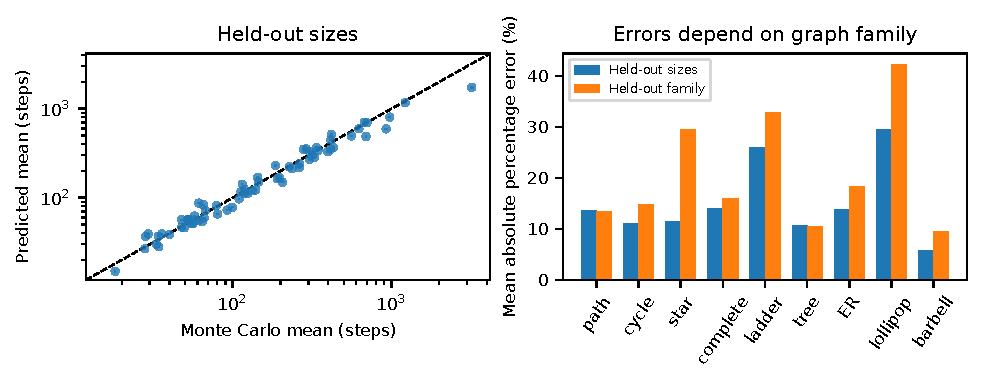
\includegraphics[width=\linewidth]{results/prediction.pdf}
\caption{Left: size-split predictions against simulated means, with horizontal 95\% Monte Carlo intervals, often smaller than the markers; the dashed line is equality. Right: four-statistic model MAPE by family under each evaluation protocol.}
\label{fig:errors}
\end{figure}

\begin{table}[t]
\centering
\caption{Four-statistic model by family. Bias is mean signed percentage error for family holdout; negative values indicate underprediction. Each deterministic family has four size-test and eight family-test graphs; tree and ER each have 20 and 40.}
\label{tab:family}
\begin{tabular}{lrrr}
\toprule
Family & Size-test MAPE & Family-test MAPE & Family-test bias\\
\midrule
Path & 13.5 & 13.5 & $-13.5$\\
Cycle & 11.1 & 14.8 & $-14.8$\\
Star & 11.6 & 29.6 & $-29.6$\\
Complete & 14.1 & 16.0 & $-6.2$\\
Ladder & 26.0 & 32.8 & $+32.8$\\
Random tree & 10.7 & 10.5 & $+1.2$\\
Connected ER & 13.9 & 18.3 & $+13.1$\\
Lollipop & 29.5 & 42.3 & $-42.3$\\
Barbell & 5.9 & 9.6 & $+6.7$\\
\bottomrule
\end{tabular}
\end{table}

Errors differ substantially across families (Figure~\ref{fig:errors}, Table~\ref{tab:family}). Every held-out lollipop is underpredicted, while every held-out ladder is overpredicted. Random trees and the particular barbells in this panel transfer better. Giving each family equal weight instead of each graph yields 15.1\% size-test and 20.8\% family-test MAPE, so the overall conclusion is not entirely due to the greater number of random graphs. Still, these averages describe this chosen panel rather than a natural distribution of small graphs.

\section{Discussion and limitations}
For these graphs, four inexpensive statistics give useful empirical predictions, with better accuracy than either baseline and errors larger than Monte Carlo noise. The family-holdout failures caution against applying the fitted formula indiscriminately: lollipops and ladders need different corrections, and stars degrade noticeably when absent from training. Degree summaries and diameter do not explicitly encode how dense regions are connected. Lollipop underprediction is consistent with missing information about bottlenecks and long excursions, but our experiment does not isolate that mechanism causally. The low error on our barbells also rules out a blanket claim that all bottleneck families fail.

The sample is small and synthetic, contains only one lollipop and barbell parameterization at each size, and tests no graphs with 2--5 vertices, no other starting distributions, and no directed or weighted graphs. The one-vertex case trivially has zero cover time and is outside the logarithmic model. Deterministic families are structurally related across sizes; the graph bootstrap is a descriptive resampling exercise, not independent evidence across graph populations. We did not compare flexible learners or resistance-based features, and make no claim that this feature set is optimal or that its coefficients are causal. A future controlled comparison could test whether a bottleneck statistic improves family transfer. The present deliverable is a reproducible smoke test, not a universal replacement for cover-time bounds.

\paragraph{Reproducibility and access.}
The accompanying \texttt{README.md} records commands, pinned dependencies, seeds, and output paths. Source code, all graph edge lists, 1,114,112 individual trajectory lengths, per-graph uncertainty estimates, and full evaluation results are included. External document access was limited to official conference template resources; no original paper answering this task or page discussing such a paper was accessed. The official NeurIPS 2024 style file is used unchanged in preprint mode; this document is not a conference submission or acceptance claim.

\bibliographystyle{plainnat}
\bibliography{references}
\end{document}
